\documentclass{article}
\usepackage[left=2cm,right=2cm,top=2cm,bottom=2cm]{geometry}
\usepackage[utf8]{inputenc}
\usepackage[german]{babel}
\usepackage{amsmath}
\usepackage{dsfont}
\usepackage[export]{adjustbox}
\usepackage{amsthm}
\usepackage{color}
\usepackage{amsfonts}
\usepackage{amssymb}
\usepackage{wasysym}
\usepackage{makeidx}
\usepackage{graphicx}
\usepackage[colorlinks=true,urlcolor=blue,linkcolor=blue]{hyperref}
\usepackage{ziffer}
\usepackage{minted}
\usepackage{xcolor}
\usepackage{framed}
\usepackage{mdframed}
\usepackage{subfiles}
\usemintedstyle{emacs}

\definecolor{purp}{HTML}{9A72AC}
\definecolor{re}{HTML}{FC6255}
\definecolor{gre}{HTML}{83C167}
\definecolor{blu}{HTML}{58C4DD}
\definecolor{shadecolor}{rgb}{0.85,0.85,0.85}
\definecolor{bg}{rgb}{0.95,0.95,0.95}
\setlength{\parindent}{0em} 

\BeforeBeginEnvironment{minted}{\begin{mdframed}[linewidth =2 ,backgroundcolor=bg , linecolor=black, linewidth=0.5]}
\AfterEndEnvironment{minted}{\end{mdframed}}

\newtheorem{defi}{Definition}
\BeforeBeginEnvironment{defi}{\begin{mdframed}[linewidth =2 ,backgroundcolor=bg , linecolor=black, linewidth=0.5]}
\AfterEndEnvironment{defi}{\end{mdframed}}

\newcommand{\bsp}{\textbf{Beispiel}:}
%\newcommand{\task}{\textbf{Aufgabe}:}

\newcommand{\bol}[1]{\textbf{#1}}
\newcommand{\q}[1]{\glqq #1\grqq}
\newcommand{\DODO}[1]{\textbf{\textcolor{red}{DODO:}} #1 \\ \begin{center}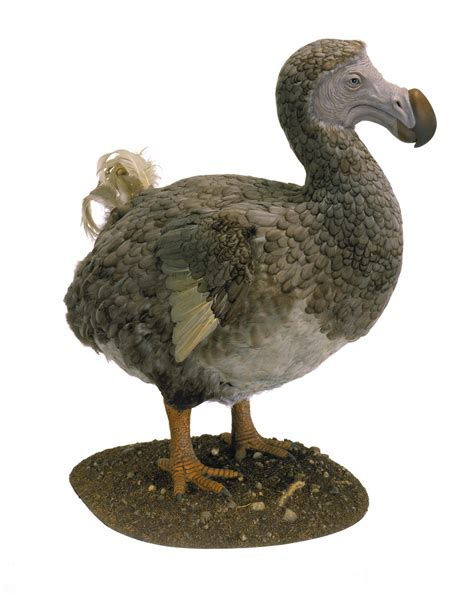
\includegraphics[scale=0.2]{../../media/dodo.jpg} \end{center}}

\newenvironment{task}[1]{
    \begin{shaded*}
    \textbf{Aufgabe #1}:
}{
    \end{shaded*}
}

\begin{document}
Es folgen die Lösungen zu den obigen Aufgaben mit Anmerkungen. \\
Zuerst die Mensch-Helferklasse
\begin{minted}{Java}
public class Human {
    private String name;
    private int age; 

    public Human(String name, int age){
        this.name = name;
        this.age = age;
    }

    public String getName(){
        return name;
    }

    public int getAge(){
        return age;
    }

    public void presentation(){
        System.out.println("I am " + name + " and I am " + age + " years old");
    }

    public boolean equals(Object o){
         if(this == o) {
             return true;
         }
         if(! (o instanceof Human)){
             return false;
         } 
         Human h = (Human) o;
         if(h.getName() == this.name && h.getAge() == this.age){
             return true;
         } else {
             return false;
         }
    }

    public boolean isGreater(Human human) {
        if(age > human.getAge()) {
            return true;
        }
        return false; 
    }
}
\end{minted}

Interessant sind in dieser Klasse nur die letzten beiden Methoden. Alle anderen sind einfache getter, setter oder Ausgabemethoden, die keine weitere spezielle Funktion haben. \\
Sucht man nach der equals(), also vergleiche() Methode, so findet man häufig den Spezialfall des Stringvergleichs. Dieser kann nur unsicher mit $==$ erfolgen, man muss equals() benutzen. \\
\begin{task}{Exkurs 1}
    Recherchieren Sie selbstständig, woran das liegt!
\end{task}
Zur Erklärung folgendes Code-Fragment als Erinnerung:
\begin{minted}{Java}
    public static void main(String[] args) {
        String x = "Hallo";
        String y = "Ha"+"llo";
        String z = hallo() + "llo";

        String a = new String("Hallo");

        System.out.println(x==y);
        System.out.println(x==z);
        System.out.println(x==a);
    }
    public static String hallo() {
        return "Ha";
    }
\end{minted}
\begin{task}{Exkurs 2}
    Welche Ausgabe erzeugen die drei obigen Vergleiche?
\end{task}
\vspace{2cm}
Der erste Vergleich liefert $true$, die anderen beiden dagegen $false$. Das liegt daran, dass ein \textbf{String} eine eigene Klasse und kein primitiver Datentyp ist (das erkennt man auch am großen ersten Buchstaben). Ein String ist \q{intern} nur ein Feld aus Zeichen, also ein $char[]$. \\
Das bedeutet aber insbesondere, dass die Variablen $x,y,z,a$ in obigem Code nur zu einem String-Objekt im Speicher zeigen und nicht direkt zu einem \q{Textinhalt}. \\
Erzeugen wir nun den String $x$, so sieht dies im Arbeitsspeicher veranschaulicht so aus: 
\begin{center}
    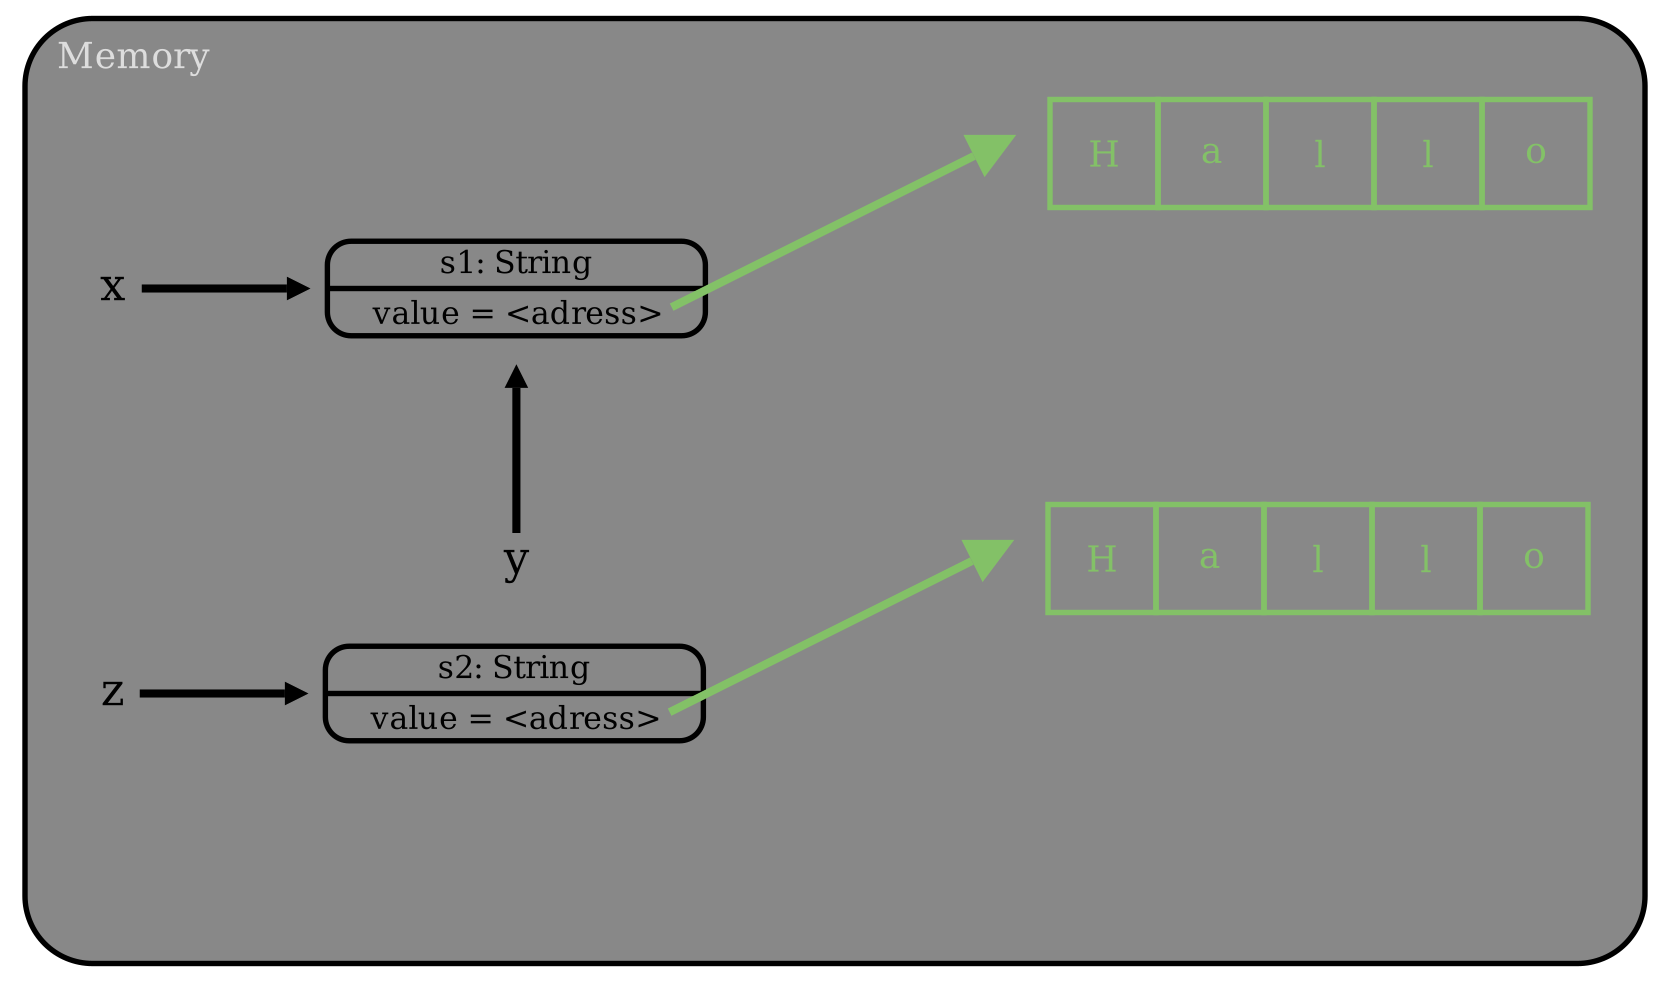
\includegraphics[scale=0.2]{../../media/string_memory.png}  
\end{center}
Der Java Compiler kann in einigen Fällen zuordnen, dass das zu erzeugende String-Objekt denselben Inhalt hat, wie ein bereits erzeugtes, z.B. im Fall der beiden Variablen $x$ und $y$, deswegen zeigen beide auf dasselbe String-Objekt. In anderen Fällen, z.B. wenn man ein neues String-Objekt erzwingt, wie bei der Variable $a$, oder wenn Funktionsaufrufe involviert sind, so ist dies nicht der Fall. Das $==$ vergleicht aber letztendlich nur, ob die beiden Zeiger der Variablen an dieselbe Adresse zeigen, das ist nur bei $x$ und $y$ der Fall. Die equals()-Methode umgeht dieses Problem, indem sie - im Falle des Strings - das zugrunde liegende Zeichenfeld vergleicht. \\
Die Definition von equals() reicht tatsählich aber noch viel tiefer. Blickt man in die Java-Dokumentation für ein Objekt (z.B. \href{https://docs.oracle.com/javase/7/docs/api/java/lang/Object.html}{Java Docs Object}), so wird hier bereits die Funktion mitsamt ihrer erwünschten Eigenschaften definiert. equals() ist außerdem für alle Java-internen Klassen (wie z.B. der String oben!) 
bereits überschrieben, d.h. der Compiler weiß, wie er zwei Strings vergleichen muss. (Den Hinweis in der Dokumentation, dass auch die hashCode Methode überschrieben werden müsste ignorieren wir aktuell geflissentlich).\\
\textbf{Zurück zum Vergleich von Menschen:}
In unserem Fall würde der Compiler nur die Referenzen zu den beiden Mensch-Objekten vergleichen, da keine weitere Implementierung vorhanden ist. Wir müssen Java also \q{beibringen}, wann wir zwei Menschen als gleich ansehen. In obigem Fall wurde das Alter und der Name als Vergleich gewählt. Es sind auch andere Implementierungen denkbar. Wichtig ist, dass die Methode vernünftig dokumentiert wird (siehe eigenes pdf), ansonsten könnte diese Vergleichsmethode andere Nutzer der Klasse verwirren. \\
Die isGreater(), also istGrößer() Methode verwendet dagegen nur das Alter der entsprechenden Person. Wenn wir das Feld später sortieren, werden die Personen unter Verwendung dieser Methode nach dem Alter sortiert. \\

Betrachten wir noch einmal einige grundlegende Methoden vor den konkreten Aufgabenlösungen in der Warteschlangenklasse:

\begin{minted}{Java}
public class MyListArray {
    private Human[] queue;
    private int count;

    public MyListArray() {
        queue = new Human[5];
        count = 0;
    }

    public void push(Human human) {
        if(count == queue.length) {
            enlargeArray();
        }
        queue[count] = human;
        count++;
    }

    private void enlargeArray() {
        Human[] newQueue = new Human[queue.length + 10];
        for(int i = 0; i < queue.length; i++){
            newQueue[i] = queue[i];
        }
        queue = newQueue;
    }

   public Human pop() {
       if(queue[0] == null) {
           return null;
       }
       Human toReturn = queue[0];
       for(int i = 0; i < queue.length -1; i++){
           if (queue[i+1] == null){
               break;
           }
           queue[i] = queue[i+1];
       }
       queue[queue.length-1] = null;
       count--;
       return toReturn;
   }

   public Human[] getQueue() {
      return queue;
   }

   public int getCount() {
      return count;
    }

    public void setCount(int count) {
        this.count = count;
    }
}
\end{minted}
\textbf{Aufgabe 3:}
Um alle Einträge auszugeben beginnen wir am nullten Eintrag und arbeiten uns bis zum Ende durch, jeweils mit dem Aufruf der dafür in der Klasse Mensch definierten Methode. 
\begin{minted}{Java}
    public void printList() {
        for(int i = 0; i < count; i++){
            queue[i].presentation();
        }
    }
\end{minted}
\textbf{Aufgabe 4:} 
Die mit Abstand einfachste Aufgabe in dieser Implementierung der Warteschlange. Wir geben nur den entsprechenden Eintrag im Feld zurück. Dabei wird angenommen, dass die erste Position im Feld dem nullten Eintrag entsprechen soll. Auch hier könnte anders programmiert werden, weswegen eine Dokumentation notwendig ist. \\
\textit{Hinweis:} Der Mensch wird durch diese Methode nicht aus der Liste entfernt, verändert man den Menschen also mit Hilfe der zurückgegebenen Referenz, so wird also auch die Liste verändert!
\begin{minted}{Java}
    public Human humanAtPosition(int position) {
        if(position >= 0 && position <= count) {
            return queue[position-1];
        } else {
            return null;
        }
    }
\end{minted}

\textbf{Aufgabe 5:}
Auch diese Aufgabe ist in dieser Warteschlange nicht besonders schwer. Die Festlegung, dass das Nicht-Enthalten eines Elements den Rückgabewert $-1$ erhält ist wiederum nicht zwingend festgelegt, sendet aber dem Benutzer ein deutliches Zeichen, dass kein solches Element vorhanden ist. Diese Methode benötigt außerdem die bereits oben besprochene überschriebene equals()-Methode für die Klasse Mensch, andernfalls wird nie ein Vergleich wahr ergeben. 
\begin{minted}{Java}
    public int searchHumanInQueue(Human human) {
        for(int i = 0; i < count; i++){
            if(queue[i].equals(human)){
                return i;
            }
        }
        return -1;
    }
\end{minted}
\textbf{Aufgabe 6:}
Hier ist sowohl eine neue iterative Implementierung möglich, als auch der Rückgriff auf die Methode aus Aufgabe 5. Wenn diese eine Zahl größer als -1 liefert, so muss es einen Index geben, an dem der entsprechende Mensch gefunden werden kann. Andernfalls muss $-1$ zurückgegeben worden sein. 
\begin{minted}{Java}
    public boolean contains(Human human) {
        for(int i = 0; i < count; i++) {
            if(human.equals(queue[i])) return true;
        }
        return false;
        /* alternatively use searchHumanInQueue:
        if(searchHumanInQueue(human)>=0) return true;
        return false;
        */
    }
\end{minted}
\textbf{Aufgabe 7:}
Auch bei dieser Methode wird davon ausgegangen, dass die erste Position in der Schlange dem nullten Eintrag im Feld entspricht. Ansonsten gibt es nur zu beachten, dass der letzte Eintrag in der Schlange händisch auf null gesetzt werden muss, da die Schlange aktuell bis zum letzten Platz besetzt sein könnte. Es wäre also möglich, dass durch die Verschiebung ein Eintrag doppelt vorkommt.
\begin{minted}{Java}
    public Human removeAtPosition(int position) {
        if(position < 0 || position > count) {
            return null;
        }
        Human toReturn = queue[position - 1];
        for(int i = position; i < queue.length - 1; i++) {
            queue[i] = queue[i+1];
        }
        queue[queue.length-1] = null;
        return toReturn;
    }
\end{minted}
\textbf{Aufgabe 8:}
Diese Aufgabe übersteigt das Pensum, das für das Abtiur von Nöten ist, die grundlegende Idee ist aber auch hier nicht schwer. Man analysiert die Listen beider Längen mit Hilfe des zugrunde liegenden Feldes und baut dann ein neues Feld auf. Danach müssen noch alle Einträge aus beiden ursprünglichen Felder hineinkopiert werden. \\
Da Kopiervorgänge viel Zeit und Speicher beanspruchen ist das Zusammenfügen, wie auch das häufige Einfügen und Löschen von Einträgen ressourcenintensiv. Listen, denen ein Feld zugrunde liegt sind also eher für Einsätze geeignet, bei denen häufig auf die Liste zugegriffen wird, sie aber nicht häufig verändert wird. 
\begin{minted}{Java}  
    public Object concatenate(MyListArray toConcat) {
        MyListArray newList = new MyListArray(this.count
            + toConcat.getCount());
        for(int i = 0; i < this.count;i++) {
            newList.getQueue()[i] = queue[i];
        }
        for(int i = 0; i < toConcat.getCount(); i++){
            newList.getQueue()[this.count + i] = toConcat.getQueue()[i];
        }
        newList.setCount(this.count+ toConcat.getCount());
        return newList;
    }
\end{minted}
\textbf{Aufgabe 9:}
Eine klassische Lösung dieses Problems besteht darin, das Element einfach anzuhängen und danach das Feld zu sortieren. Sortieralgorithmen sind ein eigenes Kapitel in der Informatik und es gibt zahllose Möglichkeiten zu sortieren. Unten stehend ist ein sogenannter InsertionSort programmiert. Jede beliebige andere Sortierung würde auch funktionieren. Eine visueller (und auditiver) Vergleich verschiedener Sortieralgorithmen findet sich zum Beispiel hier: \href{https://www.youtube.com/watch?v=kPRA0W1kECg}{Sortieralgorithmenmusik} \\
Natürlich müssen die beiden Methoden nicht separiert werden. Ein Äquivalent des InsertionSorts könnte auch direkt in der sortiertEinfügen() Methode verwendet werden. \href{https://youtu.be/pv081cVm3Xw}{Visualisierung - mit BubbleSort!}
\begin{minted}{Java}
    public void appendSorted(Human human) {
        if(queue[0] == null){
            queue[0] = human;
            count++;
        } else {
            this.push(human);
            insertionSort();
        }
    }
    
    private void insertionSort() {
        /*Divides the array in a sorted and unsorted part. It iterates over the
        unsorted part and puts the next element into the right spot in the
        sorted part thus enhancing it by one.
        */
        for(int i = 1; i < count; i++){
            //The reference to the element that shall be placed next
            Human tmp = queue[i];
            int j = i - 1; //Defines the part of the array that is sorted
            // Moves every element that is greater up one spot until it 
            //finds the right spot for the new element.
            //isGreater is necessary as it is not a primitive type.
            while(j >= 0 && queue[j].isGreater(tmp)){
                queue[j+1] = queue[j];
                j--;
            }
            //puts the new element at the found spot
            queue[j+1] = tmp;
        }
    }
\end{minted}

\vspace{2cm}

\textbf{Zusammenfassung:} \\
Die Implementierung einer Liste mit Hilfe eines Feldes hat sowohl Nachteile als auch Vorteile. Die Implementierung stützt sich im wesentlichen auf ein zugrunde liegendes Feld, dass durch die Methoden der Liste geeignet manipuliert wird. \\
\textbf{Vorteile:}
\begin{enumerate}
    \item Das Einfügen eines Elements ist effizient, wenn ausreichend Platz im Feld vorhanden ist.
    \item Der Zugriff auf ein beliebiges Element der Liste ist direkt möglich. 
\end{enumerate}
\textbf{Nachteile:}
\begin{enumerate}
    \item Das Entfernen eines Elementes zieht durch das Kopieren aller folgenden Einträge nach vorne einen großen Rechenaufwand nach sich. 
    \item Wird das Feld zu groß oder zu klein gewählt wird gegebenenfalls Speicherplatz verschwendet (viele Null-Referenzen im Feld) und es gibt keinen Platz mehr im Arbeitsspeicher oder das Feld muss häufig vergrößert werden. 
    \item Je öfter diese dynamische Größenveränderung angewandt werden muss, desto größer ist neben dem Speicher auch der Rechenaufwand.
\end{enumerate}

\textbf{Fazit:} Eine Feld-Liste bietet sich vor allem dann, wenn einmal viele Elemente eingefügt werden sollen, anschließend aber hauptsächlich auf die Elemente zugegriffen wird, ohne viele Veränderungen vorzunehmen. 

\end{document}